\documentclass[11pt,a4paper]{report}
\usepackage[T1]{fontenc}
\usepackage[latin1]{inputenc}
\usepackage{lmodern}
\usepackage{xcolor}
\usepackage{mathptmx}
\usepackage{graphicx}
\usepackage{hyperref}
\usepackage{listings}


\begin{document}




  \begin{titlepage}
    \centering
    \fontsize{22}{32}\selectfont {Virtual Machine Software Testing}\\[0.5\baselineskip]
     \fontsize{17}{27}\selectfont {Internship Report}\\[1.5\baselineskip]
    
    
    
    \fontsize{11}{20}\selectfont \it {Submitted to:} \\[0.2\baselineskip]    
    \fontsize{12}{21}\selectfont {Student Internship Bureau }\\[0.3\baselineskip]    
    \fontsize{12}{21}\selectfont  {University of York, UK }\\[0.3\baselineskip]    



\begin{figure}[h]
\centering
\parbox{5cm}{

\includegraphics[width=3.5cm]{uniLogo.png}
%\caption{First.}
\label{fig:2figsA}}
\qquad
\begin{minipage}{5cm}

\includegraphics[width=3.5cm]{rapitaLogo.png}
%\caption{Second.}
\label{fig:2figsB}
\end{minipage}
\end{figure}

\bigskip
\bigskip

 \fontsize{11}{20}\selectfont \it {Submitted by:}\\[0.2\baselineskip]    
     \fontsize{12}{21}\selectfont {Mian Asbat Ahmad, PhD. Final Year }\\[0.1\baselineskip]
      \fontsize{12}{21}\selectfont {Department of Computer Science}\\[0.1\baselineskip]    
     \fontsize{12}{21}\selectfont  {University of York, UK }\\[1\baselineskip]    


\bigskip
     
     \fontsize{12}{22}\selectfont \it {Supervisors: Jennifer Mowat and Ian Broster} \\[1\baselineskip]    
     \fontsize{12}{22}\selectfont \it {Reviewer: Dr. Manuel Oriol} \\[0.5\baselineskip]    
   %   {\fontsize{13}{23}\selectfont Ian Broster, Rapita Sytstems Ltd. (host)}\\[2\baselineskip]
    
    \bigskip \bigskip
     \fontsize{13}{23}\selectfont {Internship Start Date:  29 May, 2013 and End Date: 19 July 2013 }\\[0.5\baselineskip]
 
  \end{titlepage}
  
 
  %%%%%%%%%%%%%%%%%%%%%%%%%%%%%%%%%%%%%%%%%%%%%%%%%%%%%%%%%%%%% 
 %%%%%%%%%%%%%%%%%%%%%%%%%%%%%%%%%%%%%%%%%%%%%%%%%%%%%%%%%%%%%
  %%%%%%%%%%%%%%%%%%%%%%%%%%%%%%%%%%%%%%%%%%%%%%%%%%%%%%%%%%%%%
  %%%%%%%%%%%%%%%%%%%%%%%%%%%%%%%%%%%%%%%%%%%%%%%%%%%%%%%%%%%%%
 \newpage
 
\begin{center}
\noindent \textbf{ \fontsize{14}{22}\selectfont { Preface }}\\[0.3\baselineskip]    
\end{center}
\fontsize{11}{24}\selectfont {This report documents the work I learned and performed during my summer internship in the project ``Virtual Machine Software Testing" at Rapita Systems Ltd. York, UK. The report starts with a brief detail of the host company, working environment and the assigned project. It primarily focuses on the challenges faced and the way they were overcome during projects implementation. The report also gives an overview of the developed product with technical details.  It further highlights the additional features that when incorporated in the project will make it more productive, robust and user friendly. \\
%
\indent Finally the report highlights the importance of internship and its benefit towards my professional career. \\

\noindent Mian Asbat Ahmad}\\[0.5\baselineskip]    

 %%%%%%%%%%%%%%%%%%%%%%%%%%%%%%%%%%%%%%%%%%%%%%%%%%%%%%%%%%%%%
 %%%%%%%%%%%%%%%%%%%%%%%%%%%%%%%%%%%%%%%%%%%%%%%%%%%%%%%%%%%%%
 %%%%%%%%%%%%%%%%%%%%%%%%%%%%%%%%%%%%%%%%%%%%%%%%%%%%%%%%%%%%%
%%%%%%%%%%%%%%%%%%%%%%%%%%%%%%%%%%%%%%%%%%%%%%%%%%%%%%%%%%%%
\newpage




\begin{center}
\noindent \textbf{ \fontsize{14}{10}\selectfont {Acknowledgments}} \\[0.3\baselineskip]    
\end{center}
\fontsize{11}{24}\selectfont {It would not be possible to achieve the project completion in such a short time without the help and support I received cheerfully from whole team of Rapita Systems Ltd. The working environment at Rapita Systems is highly motivational and inspirational.
I therefore thank the whole team, however I would specially like to thank Dr. Ian Broster, Dr. Antoine Colin and  Will Lunniss for their help and support both administratively and technically.  They frankly shared their views and gave me nice ideas to work upon.  I am also highly indebted to my academic supervisor Dr. Manuel Oriol for allowing me to attain this golden opportunity and also for his valuable time to review this report.\\
\indent Last but not the least, I would like to thank the Students Internship Bureau (SIB), University of York for creating the wonderful internship opportunity, which enabled me to utilise my skills, knowledge and enthusiasm. 
\\[0.5\baselineskip] 
\noindent Author.}\\[0.5\baselineskip]    

 %%%%%%%%%%%%%%%%%%%%%%%%%%%%%%%%%%%%%%%%%%%%%%%%%%%%%%%%%%%%%
 %%%%%%%%%%%%%%%%%%%%%%%%%%%%%%%%%%%%%%%%%%%%%%%%%%%%%%%%%%%%%
%%%%%%%%%%%%%%%%%%%%%%%%%%%%%%%%%%%%%%%%%%%%%%%%%%%%%%%%%%%%%
 %%%%%%%%%%%%%%%%%%%%%%%%%%%%%%%%%%%%%%%%%%%%%%%%%%%%%%%%%%%%%
\newpage


\noindent \textbf{\fontsize{14}{22}\selectfont {Introduction:}} \\[0.2\baselineskip]    
\fontsize{11}{18}\selectfont {Automation of computer operations can be surprisingly effective and highly beneficial for any organisation. Its initial setup cost may be higher, however, a quick return on investment (QRI) outperforms it and brings the key benefits of cost reduction, productivity, availability, reliability and performance to any organisation.  Automation is particularly effective when the nature of jobs is repetitive and performed on routine basis. These simple or complex manual jobs consume unnecessary time and provide an extra burden on the staff.  \\
\indent Understanding the need and benefits of automation as a means of staying competitive in the world market, Rapita Systems Ltd. decided to automate the process of software testing.} \\[0.2\baselineskip]    
%
%
\noindent \textbf{ \fontsize{14}{22}\selectfont {Rapita Systems:}} \\[0.2\baselineskip] 
%
\indent \fontsize{11}{22}\selectfont {Rapita Systems is a local software company based in York Science Park, IT Center building, that develops software tools for on-target verification, optimisation and code coverage of critical real-time embedded systems. The technology developed by Rapita Systems Ltd is applicable to many different areas of industry and they currently have customers in the aerospace, automotive and space sectors. Please see \url{http://www.rapitasystems.com} for more information. } \\
%
%
\noindent \textbf{ \fontsize{14}{22}\selectfont {Project Details:}} \\[0.2\baselineskip] 
\fontsize{11}{28}\selectfont {I was assigned the task to set up an automated testing environment where there developed software can be automatically tested on different operating systems without any user intervention. The project should be set up using virtual machines containing various operating systems (Windows and Linux, 32 and 64 bit). Writing scripts to allow software to be automatically installed, executed and tested on those systems, with any errors reported correctly. In addition, the project will involve working with other parts of the companys test system, nightly build framework and regression test scripts.} \\
%%%%%%%%%%%%%%%%%%%%%%%

\noindent \textbf{ \fontsize{14}{22}\selectfont {Goals:}} \\[0.2\baselineskip] 
\fontsize{11}{22}\selectfont {The following goals were determined to be the top six.
\begin{enumerate}
\item Automation of install and uninstall process of the Rapita Verfication Suite (RVS) software on Windows and Linux operating systems.
\item Setup of Virtual Environment with all the major Virtual Machines (VM).
\item Establish secure and reliable communication between the entities involved.
\item Generate a detailed test report to a file and displayed in webpage on user demand.
\item Setup of front end with a simple layout and can be accessed from any client.
\item Revert all the changes after the tests are finished.
\end{enumerate}
} 

%To achieve high quality this process is repeated after minor changes in the software and where there is wastage of time the repetitive nature of the job also make it a tedious process for the staff.


To achieve the automation of the whole process the project was split up into six small categories and each one is briefly defined. \\

\noindent \textbf{ \fontsize{14}{22}\selectfont {Automation of Install and Uninstall Script:}} \\[0.2\baselineskip] 
\indent \fontsize{11}{22}\selectfont {While few easy to use commercial tools are available to automate various tasks, however, they are costly, unreliable and not flexible enough to fully meet our requirements. We therefore selected tools that may not be very friendly and may requires more technical skills to handle but they are much more reliable, highly flexible, open-source and completely free. \\
%t
\indent We selected freely available AutoIT and Expect tool to automate the install and uninstall process of RVS on Windows and Linux platform respectively. There are total 12 steps involved in RVS installation which when performed manually takes around 2 minutes to complete however with automation it can be performed in not more than 20 seconds.\\
%
\indent Automating the install and uninstall process alone saves a substantial amount of time because of the repetitive nature of the job that is performed after any change in the RVS software. Beside saving time, the automation process also relieve the staff from repeating the same process again and again.}\\

\noindent \textbf{ \fontsize{14}{22}\selectfont {Setting up Virtual Environment:}} \\[0.2\baselineskip] 
\indent \fontsize{11}{22}\selectfont {We selected Oracle Virtual Box to setup the virtual environment, which is again a free and open software. It is reliable, efficient and highly customisable to meet our requirements. It provides virtual but very close to the real environment to test software at minimum hardware cost. Snapshots and clone are additional benefits that can be highly effective in restoring the original system after the test is finished. \\
%
\indent Twelve Linux distributions (32 \& 64 bit and Desktop \& Server) and three Microsoft Windows operating systems were installed in Virtual box. These distributions were selected on the basis of their deployment at Rapita Systems clients. The detail of each Guest virtual machine is stored in the database for later use.}\\
\\
\\
\noindent \textbf{ \fontsize{14}{22}\selectfont {Secure and Reliable Intercommunication:}} \\[0.2\baselineskip] 
\indent \fontsize{11}{22}\selectfont {In the current setup of Rapita Systems, each upgraded version of the software is stored on a dedicated Software server. Similarly the Test server is used to test the software and our virtual environment is configured on the same server. Additional the guest Virtual Machines are also ran on the test server.\\
%
\indent These three system must communicate freely to perform a fully automated testing. For this purpose we created a special user Rapitabot on all the three machines and configured it in such a way that it can establish ssh connection between each other without requesting key. The same ssh connection is used to copy the software from Software server and and test scripts from Test server to Guest virtual machine. } \\

\noindent \textbf{ \fontsize{14}{22}\selectfont {Tracking test execution in Test Log: }} \\[0.2\baselineskip] 
\indent \fontsize{11}{22}\selectfont { The purpose of the whole testing system is to execute the tests and check if the tests were successful or not. Therefore a regorous reporting system is implemented to track each step of the test execution and log both the pass and fail state. \\
\indent Test logs can be accessed in two ways. It can be read on the browser by clicking the "Read Log" button or from a log file that is stored in the Test server. Logs are interactively updated and can be read in real time.} \\

\noindent \textbf{ \fontsize{14}{22}\selectfont {Design and Layout of Frond-End:}} \\[0.2\baselineskip] 
\indent \fontsize{11}{22}\selectfont {Special emphasis was given on the front-end to keep it simple, user friendly and accessible from any machine. For this reason we developed the front-end using php and HTML language to allow its access from any machine with browser software. The screenshot of the front-end is given in Figure \ref{fig:front}.

\begin{figure}[h]
\centering
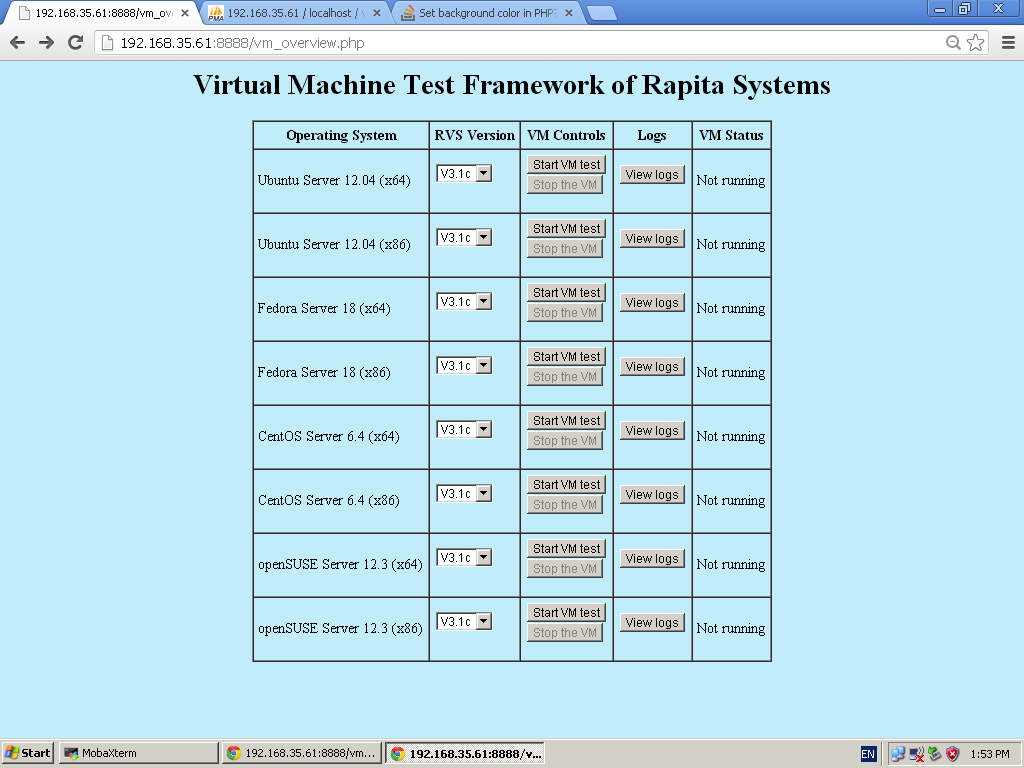
\includegraphics[width=12.5cm]{framework.png}
\caption{Front-end of Virtual Machine Test Framework of Rapita Systemss}
\label{fig:front}
\end{figure}

The front-end gets the available softwares from Software server and the Guest Virtual machines from the database to display it on a webpage. For testing the tester picks the RVS version and the operating system and click the test button. Test is executed in the background and user can click the "Read Log" button to view the test results online or tester can check the log file at a later time.}\\

\noindent \textbf{ \fontsize{14}{22}\selectfont {Revert Changes:}} \\[0.2\baselineskip] 
\indent {\fontsize{11}{22}\selectfont {Once the test is completed, it is necessary to delete all its traces to avoid any interference in the future tests. A clean up script is in placed for this reason that uninstall the installed RVS software, delete all the folders and script files and safely shutdown the Guest virtual machine.}\\

\newpage
\noindent \textbf{ \fontsize{14}{22}\selectfont {Working of the Testing System:}} \\[0.2\baselineskip] 
\indent \fontsize{11}{22}\selectfont {This section describe the step by step procedure of the system with the help of Figure \ref{fig:process}.}


\begin{figure}[h]
\centering
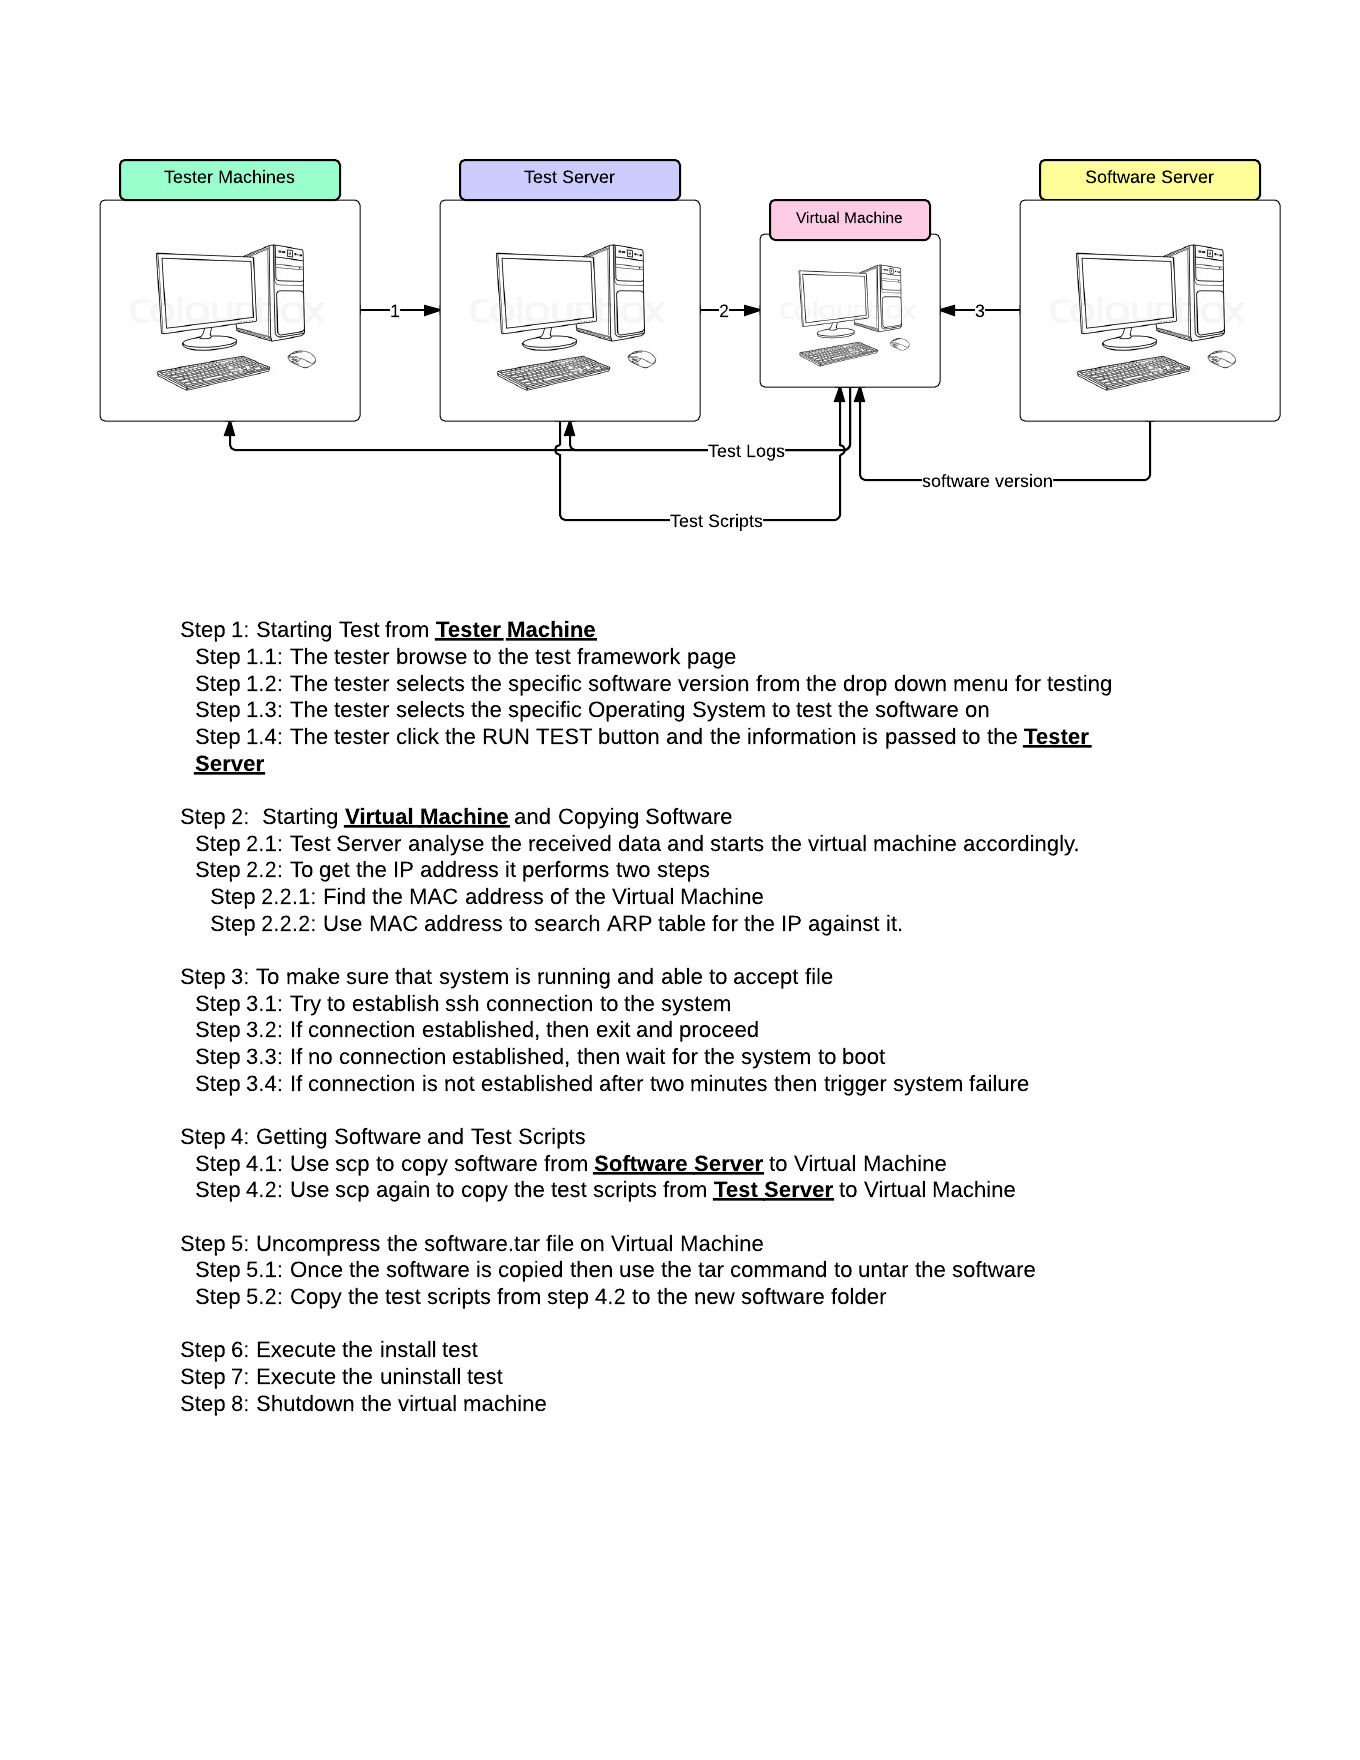
\includegraphics[width=11cm]{rapitaSystems.png}
\caption{Step by step process of the software testing}
\label{fig:process}
\end{figure}
\newpage
\noindent \textbf{ \fontsize{14}{22}\selectfont {Future Work:}} \\[0.2\baselineskip] 
\indent {\fontsize{11}{22}\selectfont {
Some additional features out of the scope of current project were identified that can be incorporated to make the system more efficient. These features include
\begin{enumerate}
\item Load balancing on test server to restrict specific number of VMs running at any time.
\item Automatic Sending the log file as email to the tester after every executed test.
\item Creating more sophisticated test suites to execute after automated installation and before uninstallation of RVS.
\item Addition of more operating systems to the virtual box.
\item Design of more attractive front-end website.
\item New webpage to install a new operating system on the fly in the virtual box according to the requirements.
\end{enumerate}
}




\noindent \textbf{ \fontsize{14}{22}\selectfont {Conclusion:}} \\[0.2\baselineskip] 
\indent \fontsize{11}{22}\selectfont {My experience of internship at Rapita Systems was great. The company has a magnificent working environment and great minds contributing to very high quality work. I learned a lot about test automation, instrumentation, data tracing and regression testing. The project I completed is very satisfactory and highly appreciated. This internship provided me the opportunity to gain hands on work experience that I couldn't get in the classroom.}\ \

\end{document}


